\section{Parametric surfaces}

\begin{itemize}
    \item A curve is a function with one parameter $\textbf{r}() = (x(t),y(t),z(t))$. 
    \begin{enumerate}
        \item Example 1. $\textbf{r}(t) = (\cos t, \sin t, 0)$, $t\in [0,2\pi]$, this is a circle in $xy$-plane ($z=0$).
        \item Example 2. $\textbf{r}(t) = (t, 2 t, 3t)$, $t\in \mathbb{R}$, this is a line going through $(0,0,0)$ with direction $\textbf{v} = (1,2,3)$. 
    \end{enumerate}
    \item A parametric surface is a function with two parameter $\textbf{r}(u,v) = (x(u,v), y(u,v), z(u,v))$, $(u,v)\in D$.
    \begin{center}
        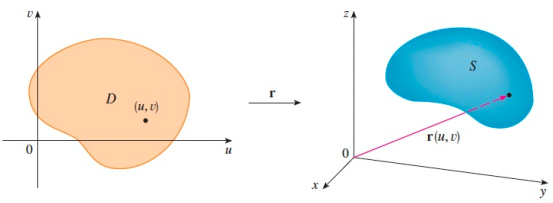
\includegraphics[scale=0.6]{images/13-parametric.png}
    \end{center}
\end{itemize}
\begin{example} $\textbf{r}(u,v) = (u,v,1-u-v)$, $(u,v)\in \mathbb{R}^2$. 
\begin{itemize}
    \item This is the plane $x+y+z = u + v + (1-u-v) = 1$.
    \item We can also view it as 
    \begin{align*}
        (u,v,1-u-v) 
        &= (0,0,1) + (u,0,-u) + (0,v,-v) = (0,0,1) + u(1,0,-1) + v(0,1,-1), \quad (u,v)\in \mathbb{R}^2.
    \end{align*}
    In this way, the plane is the one containing $(0,0,1)$ and all vectors in the planes generated by $(1,0,-1)$ and $(0,1,-1)$.
\end{itemize}
\end{example}


\begin{example} $\textbf{r}(u,v) = (2\cos u, v, 2\sin u)$, $u\in [0,2\pi], v\in \mathbb{R}$. 
\begin{itemize}
    \item Look at $x = 2\cos u, y = v, z = 2\sin u$, thus $x^2+z^2 = 4$, while $y\in \mathbb{R}$. This is a cylinder.
\end{itemize}
    \begin{center}
        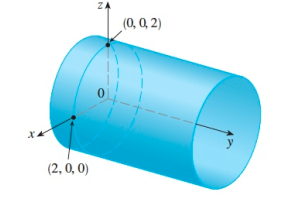
\includegraphics[scale=0.7]{images/13-ex2.png}
    \end{center}
\end{example}

\clearpage

\begin{example} $\textbf{r}(u,v) = (2\cos u, v, 2\sin u)$, $u\in \left[0,\frac{\pi}{2}\right], v\in [0,3]$. 
\begin{itemize}
    \item Look at $x = 2\cos u, y = v, z = 2\sin u$, thus $x^2+z^2 = 4$, while $y\in \mathbb{R}$. This is a cylinder.
    \item Note the angle $\theta$ in the $Oxz$-plane is $\pi/4$, thus only a quarter of the $Oxz$-plane is covered. 
\end{itemize}
    \begin{center}
        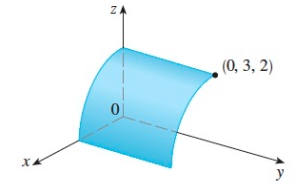
\includegraphics[scale=0.7]{images/13-ex3.png}
    \end{center}
\end{example}



\section{Parametrize a surface in $x,y,z$}
\begin{example} Find a parametric equation for $x^2+y^2 = 4, 0\leq z\leq 1$. 
\end{example}
\begin{proof} We can use polar coordinates $x = 2\cos \theta, y = 2\sin \theta$ and $0\leq z\leq 1$, thus 
\begin{equation*}
    r(\theta,z) = (2\cos \theta, 2\sin \theta, z)
\end{equation*}
The domain is $D = \{(\theta, z): 0\leq \theta \leq 2\pi, 0\leq z\leq 1\}$.
\end{proof}

\begin{example} Find a parametric equation for $z = 2\sqrt{x^2+y^2}, 0\leq z\leq 1$. 
\end{example}
\begin{proof}[Proof 1] We can just use the graph
\begin{equation*}
    r(x,y) = (x,y,z) = (x,y,2\sqrt{x^2+y^2}).
\end{equation*}
Note the condition $0\leq z\leq 1$ means $0\leq 2\sqrt{x^2+y^2}\leq 1$, thus $x^2+y^2 \leq \frac{1}{4}$. Therefore
    \begin{equation*}
        D = \left\{(x,y)\in \mathbb{R}^2: x^2+y^2 \leq \frac{1}{4}\right\}.
    \end{equation*}
\end{proof}

\begin{proof}[Proof 2] We can use polar coordinates $x = r\cos \theta, y = r\sin \theta$ and $0\leq z = 2r\leq 1$ which means $0\leq r\leq \frac{1}{2}$, thus 
\begin{equation*}
    \textbf{r}(\theta,z) = (r\cos \theta, r\sin \theta, 2r)
\end{equation*}
The domain now is 
\begin{equation*}
    D = \left\{(\theta, r): 0\leq \theta \leq 2\pi, 0\leq r\leq \frac{1}{2}\right\}.
\end{equation*}
\end{proof}


\section{Grid}
For a parametric surface $\textbf{r}(u,v)$, if we:
\begin{itemize}
    \item Fix $u=u_0$, run $v$ we get the images as a curvy grid on the surface
    \item Fix $v=v_0$, run $u$ we get the images as a curvy grid on the surface
\end{itemize}
The two direction at each point $(x_0,y_0,z_0) = r(u_0,v_0)$ form a tangent plane at that point. The two directions here are the partial derivatives
\begin{equation*}
    \textbf{r}_u \qquad \text{and} \qquad \textbf{r}_v.
\end{equation*}
The normal vector of the tangent plane is 
\begin{equation*}
    \textbf{n} = r_\textbf{u}\times r_\textbf{v} = 
    \left|
    \begin{array}{ccc}
         \textbf{i}& \textbf{j} & \textbf{k}  \\
         x_u &  y_u & z_u\\
         x_v &  y_v & z_v
    \end{array}
    \right|.
\end{equation*}
\begin{center}
    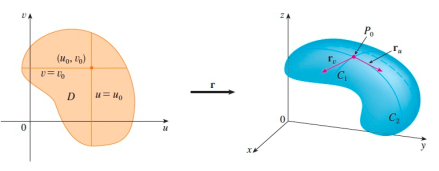
\includegraphics[scale=0.8]{images/13-grid.png}
\end{center}

\begin{example} Find the tangent plane of $x = u^2, y=v^2, z = u+2v$ at $(1,1,3)$.
\end{example}
\begin{proof} \quad 
\begin{itemize}
    \item Step 1. Solve for $(u,v)$: 
    \begin{equation*}
        \begin{cases}
            & x = u^2 = 1\\
            & y = v^2 = 1\\
            & z = u + 2v = 3
        \end{cases} \qquad\Longrightarrow\qquad \begin{cases}
            & u = \pm 1\\
            & v = \pm 1\\
            & u+2v = 3
        \end{cases} \qquad\Longrightarrow\qquad \begin{cases}
            u = 1\\
            v = 1
        \end{cases}
    \end{equation*}
    \item Step 2. Compute the partial derivatives of $\textbf{r}(u,v) = (u^2, v^2, u+2v)$
    \begin{align*}
        \textbf{r}_u = (2u, 0, 1)\\
        \textbf{r}_v = (0, 2v, 2).
    \end{align*}
    \item Step 3. Plug in the value $u=v=1$ to get 
    \begin{equation*}
        \begin{cases}
            \textbf{r}_u = (2, 0, 1)\\
            \textbf{r}_u = (0, 2, 2)
        \end{cases} 
    \end{equation*}
    \item Step 4. Compute the normal by cross product
    \begin{equation*}
        \textbf{n} = \textbf{r}_u \times \textbf{r}_v = 
        \left|
    \begin{array}{ccc}
         \textbf{i}& \textbf{j} & \textbf{k}  \\
         2 &  0 & 1\\
         0 &  2 & 2
    \end{array}
    \right| = (-2, -4, 4)
    \end{equation*}
    \item The tangent plane with normal $(-2,-4,-4)$ going through $(1,1,3)$ is
    \begin{equation*}
        \fbox{$\displaystyle 
        -2(x-1) - 4(y-1) - 4(z-3) = 0.
        $}
    \end{equation*}
\end{itemize}
\end{proof}


\begin{example} Find the tangent plane of $x = u^2+1, y=v^3+1, z = u+v$ at $(5,2,3)$.
\end{example}
\begin{proof} \quad 
\begin{itemize}
    \item Step 1. Solve for $(u,v)$: 
    \begin{equation*}
        \begin{cases}
            & x = u^2+1 = 5\\
            & y = v^3+1 = 2\\
            & z = u + v = 3
        \end{cases} \qquad\Longrightarrow\qquad \begin{cases}
            & u = 2 \\
            & v =  1.
        \end{cases} 
    \end{equation*}
    \item Step 2. Compute the partial derivatives of $\textbf{r}(u,v) = (u^2+1, v^3+1, u+v)$
    \begin{align*}
        \textbf{r}_u = (2u, 0, 1)\\
        \textbf{r}_v = (0, 3v^2, 1).
    \end{align*}
    \item Step 3. Plug in the value $u=2,  v=1$ to get 
    \begin{equation*}
        \begin{cases}
            \textbf{r}_u = (4, 0, 1)\\
            \textbf{r}_u = (0, 3, 1)
        \end{cases} 
    \end{equation*}
    \item Step 4. Compute the normal by cross product
    \begin{equation*}
        \textbf{n} = \textbf{r}_u \times \textbf{r}_v = 
        \left|
    \begin{array}{ccc}
         \textbf{i}& \textbf{j} & \textbf{k}  \\
         4 &  0 & 1\\
         0 &  3 & 1
    \end{array}
    \right| = (-3, -4, 12)
    \end{equation*}
    \item The tangent plane with normal $(-3,-4,12)$ going through $(5,2,3)$ is
    \begin{equation*}
        \fbox{$\displaystyle 
        -3(x-5) - 4(y-2) +12(z-3) = 0.
        $}
    \end{equation*}
\end{itemize}
\end{proof}